\documentclass[conference]{IEEEtran}
\IEEEoverridecommandlockouts
\usepackage[T1]{fontenc}
\usepackage{cite}
\usepackage{amsmath,amssymb}
\usepackage{graphicx}
\usepackage{booktabs}
\usepackage{multirow}
\usepackage{array}
\newcolumntype{L}[1]{>{\raggedright\arraybackslash}p{#1}}
\usepackage{xcolor}
\usepackage{tikz}
\usetikzlibrary{positioning,arrows.meta,fit,backgrounds,calc}
\usepackage[hidelinks]{hyperref}
\usepackage{url}

\definecolor{cblue}{HTML}{2A78D6}
\definecolor{corange}{HTML}{EB6834}
\definecolor{ink}{HTML}{0B0B0B}
\definecolor{ink2}{HTML}{52514E}
\definecolor{panel}{HTML}{F0EFEC}
\definecolor{bluebg}{HTML}{E6F0FC}
\definecolor{orangebg}{HTML}{FCEAE2}

\newcommand{\pp}{\,pp}

\begin{document}

\title{High NIH Accuracy Does Not Predict Transfer: Reproducing and Auditing DANet for Malaria Cell Classification}

\author{\IEEEauthorblockN{Agrapujya Lashkari and Deepanshu Mehta}
\IEEEauthorblockA{Newton School of Technology, Rishihood University\\
Sonipat, Haryana, India}}

\maketitle

\begin{abstract}
Lightweight networks for malaria cell classification report about 98\% accuracy on the NIH thin-smear dataset, but such scores do not say what a model has learned or whether it will work on another laboratory's slides. We reproduced DANet, a 2.3\,M-parameter dilated attention network, reaching 97.02\% accuracy against the published 97.95\%, and then tested one pre-registered change: stain-colour augmentation to help on unseen patients. The prediction failed (balanced accuracy $-0.04$\pp{} [$-0.22$, $+0.14$]), and patient leakage turned out to be small ($+0.26$\pp). We extended the work into an audit with dated predictions. A one-measurement ``dark-spot'' rule with no training came within 1.16\pp{} of DANet on NIH. Retraining with only a new random seed left NIH accuracy almost unchanged (SD 0.18) but moved external accuracy on MP-IDB with SD 6.63. Finally, we froze four candidates and tested them once on BBBC041 (\textit{P.~vivax}, 79{,}619 cells). A colour-transfer ensemble beat the dark-spot rule under both crop rules (AUC 0.977 vs.\ 0.909; balanced accuracy 92.1 vs.\ 61.3), against our own leading prediction. The rule kept its ranking but not its NIH threshold, calling 82\% of uninfected cells in one acquisition group. NIH accuracy mostly measures a strong simple cue, and only a frozen, untouched external test showed which approach transfers.
\end{abstract}

\begin{IEEEkeywords}
malaria, blood smear, data leakage, external validation, shortcut learning, underspecification, reproducibility
\end{IEEEkeywords}

% =====================================================================
\section{Introduction}
Light microscopy of Giemsa-stained blood smears remains the reference test for malaria, which caused an estimated 249 million cases and 608{,}000 deaths in 2022~\cite{who2023}. Reading smears is slow and depends on the reader, so automated cell classification has become a popular research target. The NIH dataset of 27{,}558 segmented red-cell crops~\cite{rajaraman2018} is its standard benchmark, and recent lightweight networks report 97--99\% accuracy on it. DANet~\cite{ali2025danet}, for example, reports 97.95\% with 2.3 million parameters.

Scores this high are hard to interpret for three reasons. First, the usual random split puts cells from the same patient in both the training and test sets, so a network can recognise a patient's slide rather than a parasite~\cite{kapoor2023,varoquaux2022}. Second, NIH crops are curated, with the parasite usually the darkest object in a pale cell, so a simple cue may suffice. Third, a model that scores well on held-out data from the same source may still behave arbitrarily on a new source, a problem known as underspecification~\cite{damour2022} and closely tied to shortcut learning~\cite{geirhos2020,zech2018}. A recent leakage-free study supports this concern: MalariaNet reached 53.2\% accuracy on BBBC041, with sensitivity 96.4\% and specificity 18.0\%~\cite{hou2026malarianet}.

This paper began as a course reproduction: reproduce one published method, then propose and test one change of our own, with the prediction written before any code. We chose DANet and hypothesised that stain-colour augmentation would help on unseen patients. That prediction failed, and the reason it failed, that leakage on NIH is small, raised a larger question: if leakage is not what makes 97\% easy, what is? We then ran a series of experiments, each with a dated prediction, that ends in a one-shot test on a dataset no model or rule had seen.

Our contributions are:
\begin{itemize}
\item a reproduction of DANet with its gap explained, and a pre-registered test of colour augmentation on unseen patients that falsified our own hypothesis (Sections~\ref{sec:repro}--\ref{sec:hyp});
\item measurements of patient and session leakage, comparisons with ResNet-18, frozen foundation-model probes and a one-measurement rule with no training, and an architecture ablation (Sections~\ref{sec:nih}--\ref{sec:ablation});
\item evidence that Grad-CAM points at parasites less reliably than ``the darkest pixel'' (Section~\ref{sec:explain}), and that a new seed alone moves external accuracy by several points (Section~\ref{sec:mpidb});
\item a frozen, hashed, one-shot external test on BBBC041 with a pre-specified outcome rule, and a failure analysis of its result (Sections~\ref{sec:bbbc}--\ref{sec:fail});
\item a complete record of predictions, including the many that failed (Section~\ref{sec:record}).
\end{itemize}

% =====================================================================
\section{Related Work}
\textbf{Malaria cell classification.} Rajaraman \textit{et al.} released the NIH dataset and showed that ImageNet-pretrained CNNs reach about 98\% accuracy~\cite{rajaraman2018}, later improved with ensembles~\cite{rajaraman2019}. Compact CNNs target phones and microcontrollers~\cite{fuhad2020}, and DANet adds dilated attention blocks at 2.3\,M parameters~\cite{ali2025danet}. EMFE showed that a five-feature model built on green-channel spots reaches AUC 0.9765 on NIH under patient-grouped validation~\cite{alkafi2026emfe}, which suggests that much of the task is simple.

\textbf{Evaluation pitfalls.} Leakage between training and test data is a leading cause of irreproducible results in machine-learning science~\cite{kapoor2023}, and medical imaging adds dataset-specific failures~\cite{varoquaux2022}. Zech \textit{et al.} showed that pneumonia models learn hospital-specific signals and lose accuracy at new sites~\cite{zech2018}. MalariaNet evaluated without slide leakage and reported large drops on MP-IDB and BBBC041~\cite{hou2026malarianet}.

\textbf{Stain and robustness.} Colour augmentation and stain normalisation are standard remedies for stain variation in computational pathology~\cite{tellez2019}; Reinhard transfer matches colour statistics in LAB space~\cite{reinhard2001}. Shortcut learning~\cite{geirhos2020} and underspecification~\cite{damour2022} explain why such remedies can help on one dataset and not another.

\textbf{Explanations and foundation models.} Grad-CAM~\cite{selvaraju2017} is the most common explanation in malaria papers, but saliency maps can look plausible without reflecting the model~\cite{adebayo2018}. Self-supervised backbones such as DINOv2~\cite{oquab2023}, the haematology model DinoBloom~\cite{koch2024} and the red-cell model RedDino~\cite{zedda2025} offer frozen features as strong references.

\textbf{Pre-registration.} Writing hypotheses and analyses down before seeing data separates confirmatory from exploratory findings~\cite{nosek2018}. We applied this to every experiment after the first milestone.

% =====================================================================
\section{Materials and Methods}

\begin{figure*}[t]
\centering
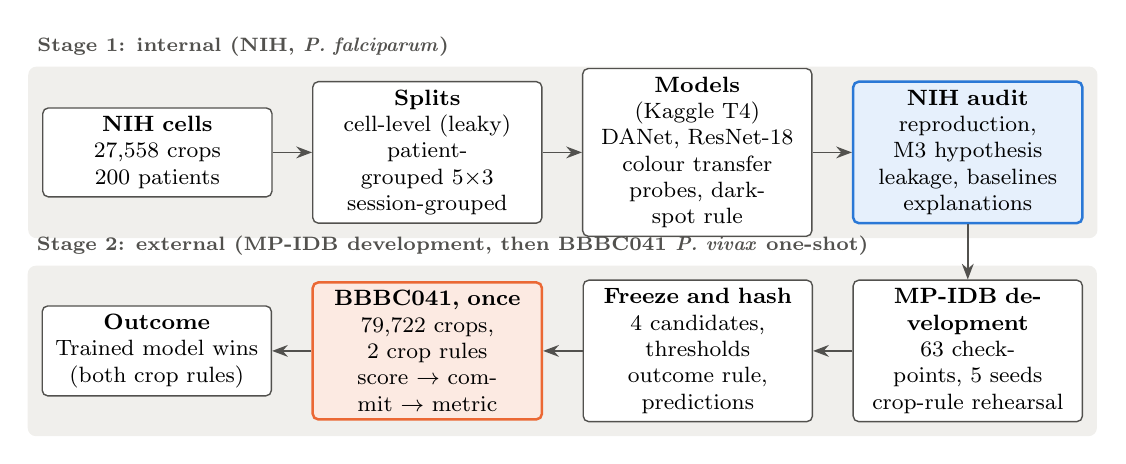
\begin{tikzpicture}[
  font=\footnotesize, node distance=4mm and 5mm,
  box/.style={draw=ink2, line width=0.5pt, rounded corners=2pt, fill=white, align=center, inner sep=3pt, minimum height=11mm, text width=27mm},
  hl/.style={box, draw=cblue, line width=0.9pt, fill=bluebg},
  ho/.style={box, draw=corange, line width=0.9pt, fill=orangebg},
  arr/.style={-{Stealth[length=2mm]}, line width=0.6pt, ink2},
  lab/.style={font=\scriptsize\bfseries, text=ink2, anchor=south west}]
\node[box] (nih) {\textbf{NIH cells}\\27{,}558 crops\\200 patients};
\node[box, right=of nih] (split) {\textbf{Splits}\\cell-level (leaky)\\patient-grouped 5$\times$3\\session-grouped};
\node[box, right=of split] (train) {\textbf{Models} (Kaggle T4)\\DANet, ResNet-18\\colour transfer\\probes, dark-spot rule};
\node[hl, right=of train] (audit) {\textbf{NIH audit}\\reproduction, M3 hypothesis\\leakage, baselines\\explanations};
\node[box, below=7mm of audit] (mp) {\textbf{MP-IDB development}\\63 checkpoints, 5 seeds\\crop-rule rehearsal};
\node[box, left=of mp] (freeze) {\textbf{Freeze and hash}\\4 candidates, thresholds\\outcome rule, predictions};
\node[ho, left=of freeze] (bb) {\textbf{BBBC041, once}\\79{,}722 crops, 2 crop rules\\score $\rightarrow$ commit $\rightarrow$ metric};
\node[box, left=of bb] (out) {\textbf{Outcome}\\Trained model wins\\(both crop rules)};
\draw[arr] (nih) -- (split); \draw[arr] (split) -- (train); \draw[arr] (train) -- (audit);
\draw[arr] (audit) -- (mp); \draw[arr] (mp) -- (freeze); \draw[arr] (freeze) -- (bb); \draw[arr] (bb) -- (out);
\begin{scope}[on background layer]
\node[fill=panel, rounded corners=3pt, inner sep=5pt, fit=(nih)(audit)] (p1) {};
\node[fill=panel, rounded corners=3pt, inner sep=5pt, fit=(out)(mp)] (p2) {};
\end{scope}
\node[lab] at (p1.north west) {Stage 1: internal (NIH, \textit{P.~falciparum})};
\node[lab] at (p2.north west) {Stage 2: external (MP-IDB development, then BBBC041 \textit{P.~vivax} one-shot)};
\end{tikzpicture}
\caption{Study design. Every experiment had a prediction written before it ran. MP-IDB was used repeatedly for development; BBBC041 was opened only after all four candidates, the outcome rule and the score hashes were fixed.}
\label{fig:design}
\end{figure*}

\subsection{Datasets}
Table~\ref{tab:data} lists the three datasets, and Fig.~\ref{fig:examples} shows random crops from each. \textbf{NIH}~\cite{rajaraman2018} provides cell crops from 200 patients after merging one patient recorded under two microscope IDs. \textbf{MP-IDB}~\cite{loddo2019mpidb} provides field images with expert parasite masks; we segmented cells with Cellpose~\cite{stringer2021}, set the background to black as in NIH, and excluded border, size-outlier and overlapping cells. \textbf{BBBC041}~\cite{hung2017,ljosa2012} provides \textit{P.~vivax} field images with expert boxes and stages. We cropped every annotated cell, excluding border and ``difficult'' boxes and red-cell boxes overlapping a parasite box, and kept the natural prevalence of 3.05\%. Its images form two acquisition groups, identifiable by format and size (1{,}208 PNG and 120 JPG). Because BBBC041 provides boxes rather than masks, we built crops with two rules: an inscribed ellipse and Otsu thresholding of the green channel.

\begin{table}[t]
\caption{Datasets and their roles}
\label{tab:data}
\centering
\footnotesize
\setlength{\tabcolsep}{3pt}
\begin{tabular}{@{}llll@{}}
\toprule
Dataset & Species & Role & Cells (parasitized) \\
\midrule
NIH~\cite{rajaraman2018} & \textit{P.~falciparum} & train, internal test & 27{,}558 (13{,}779) \\
MP-IDB~\cite{loddo2019mpidb} & \textit{P.~falciparum} & external development & 14{,}468 (963) \\
BBBC041~\cite{hung2017} & \textit{P.~vivax} & one-shot test & 79{,}619 (2{,}425)$^{*}$ \\
\bottomrule
\end{tabular}\\[2pt]
\raggedright\scriptsize $^{*}$Plus 103 leukocytes, scored as hard negatives only. MP-IDB: 104 images; BBBC041: 1{,}328 images.
\end{table}

\begin{figure*}[t]
\centering
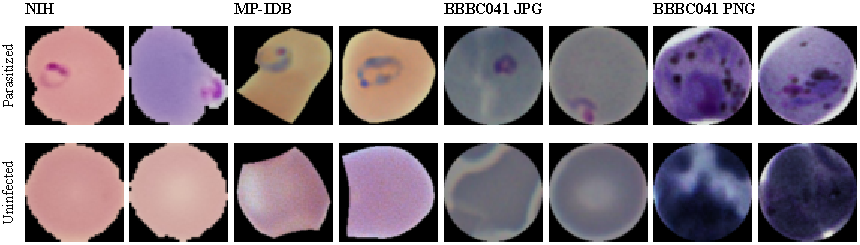
\includegraphics[width=\textwidth]{figures/fig_examples.pdf}
\caption{Random crops (fixed seed) from each source. Top: parasitized; bottom: uninfected. NIH and MP-IDB are \textit{P.~falciparum}; BBBC041 is \textit{P.~vivax} with two acquisition groups whose stain and contrast differ sharply. BBBC041 images are CC BY-NC-SA 3.0, from the Broad Bioimage Benchmark Collection~\cite{ljosa2012}.}
\label{fig:examples}
\end{figure*}

\subsection{Splits}
We used three NIH splits, each fixed and hashed before training. \textbf{Leaky:} a random cell-level 70/10/20 split (seed 42), our reconstruction of DANet's unseeded split. \textbf{Patient-grouped:} five folds over patients, repeated three times. Patients are stratified as healthy-only or one of three tertiles of parasitized-cell count, and each test fold holds 10 patients from each stratum. \textbf{Session-grouped:} patients sharing an imaging date (from file names) were linked into 50 blocks, and whole blocks were assigned to folds, so training, validation and test share no date. Date is a proxy for session.

\subsection{Baseline: reproducing DANet}
DANet-S~\cite{ali2025danet} stacks dilated attention blocks with InstanceNorm and a channel gate, for 2.31\,M parameters and 0.83\,GFLOPs at 224\,px. The released code did not run as published: it failed on import and had a 32-way output layer for a two-class task. The learning rate in the paper's hyperparameter table (0.01) did not train. We used the setting we found that trained: RMSprop with a one-cycle schedule, maximum learning rate 0.001, batch size 64, 224\,px inputs, 75 epochs for the reproduction and 50 for all audit runs (reduced after a timing test), negative log-likelihood loss, rotation ($\pm15^\circ$) and flip ($p=0.2$) augmentation, keeping the checkpoint with the lowest validation loss. The released code also differs from the paper's description: it uses a softmax gate over channels, cascaded dilations and InstanceNorm, while the paper describes a sigmoid gate, parallel dilations and LayerNorm. Our main model (E1) follows the code. We also trained a paper-faithful variant with LayerNorm (E8b) and the same variant with InstanceNorm (E8c); these are the ``three DANet variants'' below. We also trained ResNet-18~\cite{he2016} (ImageNet weights, AdamW, 128\,px, 15 epochs) as a generic reference. All models were trained on Kaggle T4 GPUs.

\subsection{Our hypothesis (Milestone 3)}
\label{sec:hypdef}
Before writing any new code, we measured that patient identity explains 74--90\% of the variance in a cell's mean colour, and that every test patient in the leaky split also contributes training cells. We therefore hypothesised that \emph{stain-colour augmentation} (ColorJitter: brightness 0.1, contrast 0.1, saturation 0.5, hue 0.1), calibrated to the measured between-patient spread, would remove the slide's colour fingerprint as a shortcut and improve accuracy on unseen patients. This was the single change. The prediction, submitted on 2026-10-05, was: against the patient-split baseline (B1), sensitivity $+0.5$ to $+1.5$\pp{} and balanced accuracy $+0.3$ to $+1.0$\pp{}, with no gain in a leaky-split control (C). The hypothesis would be falsified if the augmented model (H) did not beat B1 on both sensitivity and balanced accuracy.

\subsection{Audit experiments}
After the hypothesis test we registered a further series of experiments, each with a prediction written before it ran: patient and session leakage; ResNet-18 and frozen-probe references; a one-measurement rule; explanation validity across five checkpoints; between-checkpoint and between-seed variance on MP-IDB; training-time colour transfer; and the BBBC041 test.

\textbf{Dark-spot rule.} For a crop with zero background, resized to 128\,px, the score is $(m - \min g)/m$, where $g$ is the Gaussian-smoothed green channel ($\sigma = 1.5$) inside the cell eroded by 4\,px, and $m$ its median. A cell is called parasitized when the score is at least 0.3047, the value that maximises balanced accuracy on NIH. The rule has one fitted number. Because we designed it after inspecting MP-IDB explanations, its MP-IDB results are exploratory.

\textbf{Colour transfer.} During training only, with probability 0.5, a cell is recoloured to another training patient's foreground statistics by Reinhard transfer in LAB space~\cite{reinhard2001}.

\textbf{Probes.} Logistic regression on frozen DINOv2-S~\cite{oquab2023}, DinoBloom-S~\cite{koch2024} and RedDino-S~\cite{zedda2025} embeddings, fitted on NIH. RedDino was not used externally, because it was trained on data that may include BBBC041.

\subsection{One-shot external test on BBBC041}
\label{sec:protocol}
Four candidates were frozen, and their code and checkpoint hashes recorded, before any BBBC041 score existed: (1) the dark-spot rule at 0.3047; (2) an ensemble of five E1 DANets (mean logit $\geq 0$); (3) a colour-transfer ensemble of 15 DANets of three variants and five ResNet-18s; and (4) DINOv2 and DinoBloom probes, as descriptive references. Nothing was refitted, recalibrated or re-thresholded on BBBC041. With $\Delta$ = candidate 3 minus candidate 1, AUC and balanced accuracy were co-primary, each with a 97.5\% image-clustered bootstrap CI (5{,}000 draws). The first matching outcome in this order decided: \emph{no transfer} (both AUCs below 0.80); \emph{feature holds} (AUC upper bound $\le +0.01$ and balanced-accuracy upper bound $\le +2$\pp); \emph{trained model wins} (both lower bounds above those margins); \emph{ranking and threshold disagree}; otherwise \emph{inconclusive}. Because rehearsal on MP-IDB showed that the crop rule alone could change the outcome, we decided before scoring to apply the rule to both crop rules and to accept an outcome only if both agreed. Scores were saved, hashed and committed before any label was read.

\subsection{Statistics}
Balanced accuracy (BACC) was the primary metric, with sensitivity (SE), specificity (SP) and AUC; the decision threshold was 0.5 unless stated. CIs come from bootstrap resampling of whole patients on NIH and whole images externally, so correlated cells move together. An A/A test between runs that differ only in seed gave a noise floor of 0.29\pp{} BACC on NIH (2.8 times the paired standard error), which we call the minimum detectable effect (MDE). It is a practical-relevance threshold, not a power calculation: an effect below it can still have a CI that excludes zero, and we report such effects as real but too small to matter. Seed variance used a pooled within-fold SD with a chi-square CI.

\subsection{Predictions and corrections}
Every prediction is dated. The Milestone~3 hypothesis was submitted to our course on 2026-10-05; later predictions are dated in our repository and are self-reported. Corrections are added above the original text and never replace it, and failed predictions remain on record (Table~\ref{tab:record}).

% =====================================================================
\section{Results}

\subsection{Reproduction}
\label{sec:repro}
On the paper's random split our reproduction reached 97.02\% accuracy and AUC 0.9945 (Table~\ref{tab:repro}). This is 0.93\pp{} below the headline 97.95\%, but inside the paper's own five-fold range (96.97--97.42\%). The gap is concentrated in sensitivity (96.30 vs.\ 98.07\%): we missed 102 parasitized cells. Likely causes are the repaired code, the learning-rate choice and the unseeded split in the released code; we could not separate them.

\begin{table}[t]
\caption{DANet reproduction on the NIH random split}
\label{tab:repro}
\centering
\footnotesize
\setlength{\tabcolsep}{3pt}
\resizebox{\columnwidth}{!}{%
\begin{tabular}{@{}lcccccc@{}}
\toprule
 & ACC & PR & SE & SP & F1 & AUC \\
\midrule
Paper~\cite{ali2025danet}, single split & 97.95 & 97.76 & 98.07 & 97.87 & 97.86 & 0.98 \\
Paper, 5-fold mean & 97.25 & 97.21 & 97.20 & -- & 97.20 & -- \\
Ours (seed 42) & 97.02 & 97.72 & 96.30 & 97.75 & 97.00 & 0.9945 \\
\bottomrule
\end{tabular}}
\end{table}

\subsection{The colour-augmentation hypothesis was falsified}
\label{sec:hyp}
Table~\ref{tab:hyp} shows the pre-registered rows. Moving to unseen patients (B1) cost only 0.23\pp{} BACC, far less than the 1--2.5\pp{} we predicted. ColorJitter (H) did not help: H minus B1 was $-0.04$\pp{} [$-0.22$, $+0.14$] in BACC and $+0.06$\pp{} [$-0.17$, $+0.29$] in SE, and both CIs exclude the predicted ranges. The between-split SD also failed to shrink (0.52 to 0.74). The control behaved as predicted. Our ``why we might be wrong'' note had anticipated one reason: DANet normalises every block with InstanceNorm, which already removes much of a global stain shift. A stronger colour method, transfer between patients' statistics, also left grouped BACC unchanged ($96.78 \to 96.78$). On NIH, colour is not where the remaining errors are.

\begin{table}[t]
\caption{Milestone 3 rows: prediction vs.\ result (BACC, \%)}
\label{tab:hyp}
\centering
\footnotesize
\setlength{\tabcolsep}{3pt}
\resizebox{\columnwidth}{!}{%
\begin{tabular}{@{}llccc@{}}
\toprule
Row & Configuration & Predicted & BACC & SE \\
\midrule
B0 & baseline, leaky split & measured & 97.03 & 96.30 \\
B1 & baseline, patient split & $-1$ to $-2.5$ vs.\ B0 & 96.80$\pm$0.52 & 96.08 \\
H & + ColorJitter, patient split & $+0.3$ to $+1.0$ vs.\ B1 & 96.72$\pm$0.74 & 96.05 \\
C & + ColorJitter, leaky split & within $\pm0.3$ of B0 & 96.84 & 95.72 \\
\midrule
\multicolumn{2}{@{}l}{H $-$ B1, paired (95\% CI)} & & $-0.04$ [$-0.22$, $0.14$] & $+0.06$ \\
\bottomrule
\end{tabular}}\\[2pt]
\raggedright\scriptsize Patient split: 3 seeds, 40 test patients each; mean $\pm$ SD. AUC was 0.994 in every row.
\end{table}

\subsection{What NIH measures}
\label{sec:nih}
With five patient-grouped folds repeated three times, DANet reached BACC $96.71 \pm 0.08$ (SE 95.91, SP 97.51, AUC 0.992), against $96.96 \pm 0.20$ on leaky splits: a leakage gap of $+0.26$\pp, below the MDE. Session-held-out folds gave $+0.24$\pp{} [$-0.06$, $+0.59$], again below the MDE; with one repeat we do not claim that session leakage is absent. Fig.~\ref{fig:forest} collects these comparisons. DANet's margin over ResNet-18 was within noise, and frozen probes came within 0.3--0.7\pp. The dark-spot rule reached AUC 0.981 and BACC 95.62 with no training. DANet was reliably better, by $+1.16$\pp{} [$0.90$, $1.45$], with 888 errors against 1{,}208 and fewer false positives on healthy patients (1.96\% vs.\ 3.63\%). DANet's training therefore buys about one point over one measurement, and that point is real. Fig.~\ref{fig:confusion}(a) shows DANet's NIH confusion matrix.

\begin{figure}[t]
\centering
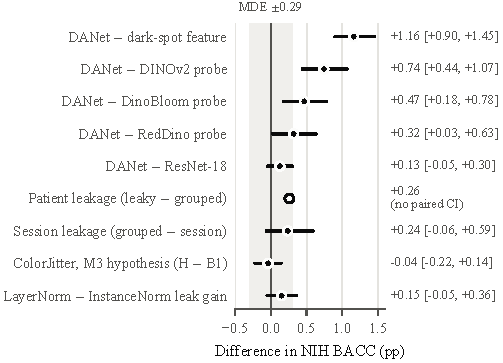
\includegraphics[width=\columnwidth]{figures/fig_forest.pdf}
\caption{Paired differences in NIH balanced accuracy, with patient-cluster bootstrap 95\% CIs. The shaded band is the 0.29\pp{} minimum detectable effect. Every effect on NIH is within about one point; the patient-leakage gap compares independent runs, so it has no paired CI.}
\label{fig:forest}
\end{figure}

\subsection{Architecture ablation}
\label{sec:ablation}
To see which part of DANet earns its accuracy, we registered two single-change ablations on the same grouped folds (repeat 0, one seed each; Table~\ref{tab:ablation}). Removing the attention path from every Dilated Attention Block, which leaves only each block's 1$\times$1 projection and 42{,}778 parameters (1.9\% of DANet), cost $-0.74$\pp{} BACC [$-1.08$, $-0.43$], lower on all five folds and almost entirely through sensitivity ($-1.47$\pp; SP $-0.01$). Replacing the average-pool head with a max pool cost $-0.19$\pp{} [$-0.37$, $-0.01$]: a CI that excludes zero, but an effect below the MDE. The attention blocks are therefore worth a real but small part of a point, and a network 54 times smaller still reaches 96.0\%.

\begin{table}[t]
\caption{Architecture ablation on NIH (grouped repeat 0, pooled out-of-fold)}
\label{tab:ablation}
\centering
\footnotesize
\setlength{\tabcolsep}{3pt}
\resizebox{\columnwidth}{!}{%
\begin{tabular}{@{}lrcccc@{}}
\toprule
Model & Params & BACC & SE & SP & AUC \\
\midrule
DANet E1 (unchanged) & 2{,}310{,}842 & 96.78 & 96.01 & 97.55 & 0.9924 \\
No attention (E13a) & 42{,}778 & 96.04 & 94.54 & 97.54 & 0.9893 \\
Max-pool head (E13b) & 2{,}310{,}842 & 96.59 & 95.78 & 97.41 & 0.9932 \\
\midrule
\multicolumn{2}{@{}l}{E13a $-$ E1 (95\% CI)} & $-0.74$ [$-1.08$, $-0.43$] & $-1.47$ & $-0.01$ & $-0.003$ \\
\multicolumn{2}{@{}l}{E13b $-$ E1 (95\% CI)} & $-0.19$ [$-0.37$, $-0.01$] & $-0.23$ & $-0.14$ & $+0.001$ \\
\bottomrule
\end{tabular}}\\[2pt]
\raggedright\scriptsize Paired patient-cluster bootstrap. One training seed per arm.
\end{table}

\subsection{What explanations show}
\label{sec:explain}
On MP-IDB, where experts mask each parasite, we asked how often a pointer lands on the parasite in correctly detected cells. Across all 15 checkpoints (three DANet variants, five folds each), the darkest smoothed pixel, chosen with no model at all, hit the parasite more often than the peak of Grad-CAM~\cite{selvaraju2017} (Fig.~\ref{fig:explain}). Darkest pixel minus Grad-CAM was $+27.3$\pp{} [15.8, 38.0] for DANet. Grad-CAM was also unstable across folds: the paper-faithful InstanceNorm variant (E8c) hit about 90\% on two folds and 8--16\% on three, so our earlier single-checkpoint result was not representative. These maps show dependence on a dark object; they give no evidence of learned parasite morphology~\cite{adebayo2018}.

\begin{figure}[t]
\centering
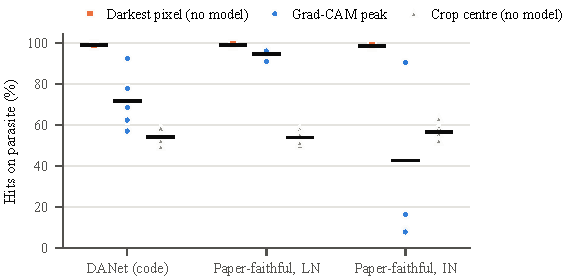
\includegraphics[width=\columnwidth]{figures/fig_explain.pdf}
\caption{Share of true positives on MP-IDB where each pointer hits the annotated parasite (dilated mask). Dots: five folds; bars: means. The no-model darkest pixel beat Grad-CAM on 15 of 15 checkpoints.}
\label{fig:explain}
\end{figure}

\subsection{External development on MP-IDB}
\label{sec:mpidb}
On MP-IDB, E1 DANet scored BACC $72.75 \pm 8.41$ across five folds, and no architecture ranking survived five checkpoints per variant. Because each fold changes both the training patients and the model, we isolated the seed: two randomly drawn folds were retrained with four new seeds each. Fig.~\ref{fig:seeds} shows the result. The same ten checkpoints had a pooled seed SD of 0.18 on their NIH test folds and 6.63 [4.48, 12.71] on MP-IDB. On fold 3, two seeds differed by 0.15\pp{} on NIH and by 13.7\pp{} on MP-IDB. NIH could not have warned of this, and a single checkpoint is a poor unit of external evidence. Training-time colour transfer raised MP-IDB BACC by $+7.05$\pp{} [4.35, 9.65] and AUC by $+0.059$, while test-time Reinhard normalisation lowered BACC by 18.75\pp{} [15.03, 22.73] by suppressing sensitivity. The registered protocol paired a field-level source standard deviation with a cell-level target one; a rerun with matched definitions (unregistered) was still $-15.37$\pp{} [$-18.73$, $-12.29$], so the flaw explains only part of the harm.

\begin{figure}[t]
\centering
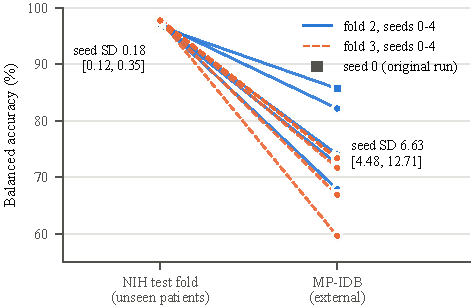
\includegraphics[width=\columnwidth]{figures/fig_seeds.pdf}
\caption{Underspecification. Ten DANet checkpoints share their training patients within each fold and differ only in the random seed. On NIH their pooled within-fold SD is 0.18\pp{} (largest within-fold range 0.64); on MP-IDB they span 59.6--85.7\%.}
\label{fig:seeds}
\end{figure}

\subsection{One-shot test on BBBC041}
\label{sec:bbbc}
Both crop rules were scored in full: 79{,}722 crops each, with order, file hashes and missing values checked, no rescoring, and both score manifests committed before any metric. Table~\ref{tab:bbbc} gives the results. Candidate 3 minus candidate 1 was $+0.068$ [0.053, 0.084] AUC and $+30.8$\pp{} [29.8, 31.9] BACC on ellipse crops, and $+0.074$ [0.058, 0.090] and $+24.8$\pp{} [23.7, 25.7] on Otsu crops. Both lower bounds cleared their margins under both crop rules, so the registered outcome is \textbf{trained model wins}. We had given this outcome 15\% and expected the feature to hold. Fig.~\ref{fig:bbbc}(a,b) shows that the ranking of the two ensembles is close, and that the operating points differ far more than the curves.

\begin{table}[t]
\caption{BBBC041 one-shot results at frozen NIH thresholds}
\label{tab:bbbc}
\centering
\footnotesize
\setlength{\tabcolsep}{4pt}
\resizebox{\columnwidth}{!}{%
\begin{tabular}{@{}lccccc@{}}
\toprule
Candidate & AUC & BACC & SE & SP & PPV \\
\midrule
\multicolumn{6}{@{}l}{\textit{Ellipse crops}} \\
1. Dark-spot rule & 0.909 & 61.3 & 99.7 & 22.9 & 3.9 \\
2. DANet E1 ensemble & 0.966 & 87.9 & 98.4 & 77.4 & 12.0 \\
3. Colour-transfer ensemble & \textbf{0.977} & \textbf{92.1} & 92.3 & 91.9 & 26.4 \\
4. DINOv2 probe & 0.936 & 77.3 & 97.2 & 57.5 & 6.7 \\
4. DinoBloom probe & 0.694 & 63.6 & 81.3 & 45.9 & 4.5 \\
\midrule
\multicolumn{6}{@{}l}{\textit{Otsu crops}} \\
1. Dark-spot rule & 0.906 & 64.4 & 99.3 & 29.6 & 4.2 \\
2. DANet E1 ensemble & 0.975 & 81.8 & 99.8 & 63.8 & 8.0 \\
3. Colour-transfer ensemble & \textbf{0.980} & \textbf{89.2} & 98.9 & 79.5 & 13.2 \\
\bottomrule
\end{tabular}}\\[2pt]
\raggedright\scriptsize 79{,}619 cells, 3.05\% parasitized; PPV at this natural prevalence. $\Delta$ (3 $-$ 1), 97.5\% image-clustered CIs: ellipse AUC $+0.068$ [0.053, 0.084], BACC $+30.8$ [29.8, 31.9]; Otsu AUC $+0.074$ [0.058, 0.090], BACC $+24.8$ [23.7, 25.7].
\end{table}

\begin{figure*}[t]
\centering
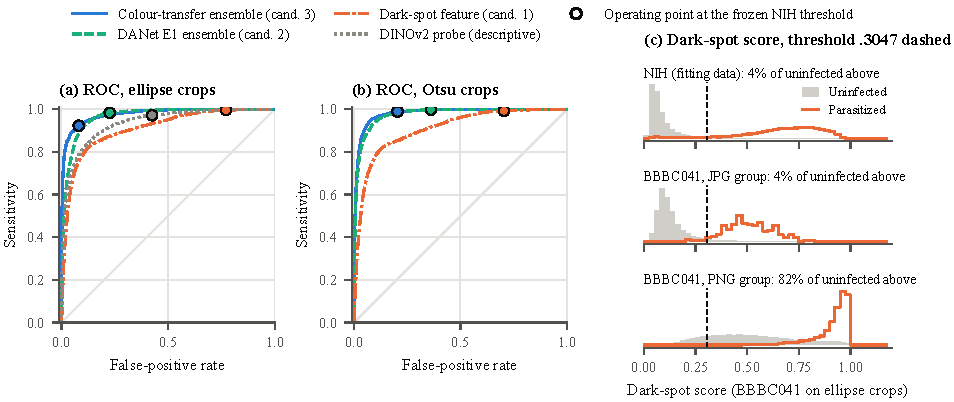
\includegraphics[width=\textwidth]{figures/fig_bbbc041.pdf}
\caption{BBBC041. (a, b) ROC curves with each candidate's operating point at its frozen NIH threshold. The two ensembles rank cells similarly; their thresholds differ. (c) Dark-spot scores by source: the NIH threshold separates the classes on NIH and on BBBC041's JPG group, but 82\% of uninfected PNG cells score above it.}
\label{fig:bbbc}
\end{figure*}

\begin{figure*}[t]
\centering
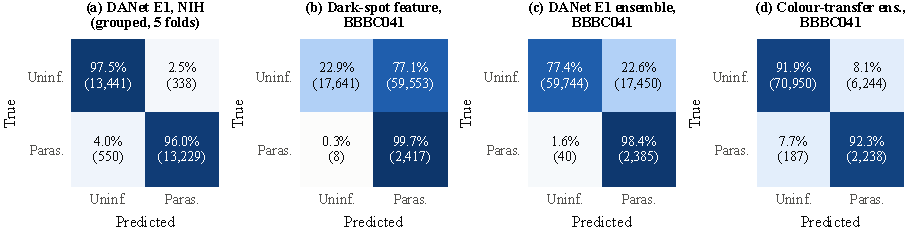
\includegraphics[width=\textwidth]{figures/fig_confusion.pdf}
\caption{Confusion matrices, row-normalised (counts in brackets). (a) DANet on unseen NIH patients, pooled over five folds. (b--d) The three BBBC041 candidates on ellipse crops at their frozen thresholds. The dark-spot rule calls almost every cell parasitized; the colour-transfer ensemble is the only candidate with balanced errors.}
\label{fig:confusion}
\end{figure*}

\subsection{Failure analysis}
\label{sec:fail}
\textbf{Where the rule failed.} On the JPG group (120 images) the dark-spot rule reached AUC 0.990 and BACC 96.4, close to candidate 3 (0.999 and 98.4). On the PNG group (1{,}208 images, 93\% of cells) its AUC was 0.957 but its BACC was 58.9: uninfected PNG cells have a median score of 0.486 against the threshold of 0.3047 (Fig.~\ref{fig:bbbc}(c)). Even a threshold chosen on BBBC041 itself would have raised its BACC only to 84.8, because the two groups need different thresholds (exploratory). Candidate 3's fixed threshold was close to its best case (92.1 vs.\ 92.3). The rule's failure is a threshold failure, the same high-sensitivity, low-specificity pattern MalariaNet reported on this dataset~\cite{hou2026malarianet}, although its accuracy of 53.2\% implies a much higher parasitized share than our natural 3.05\%, so the numbers are not directly comparable.

\textbf{Per-class recall.} Table~\ref{tab:stage} breaks sensitivity down by stage. The rule caught nearly every parasite, because it called nearly everything. Candidate 3's weakest class was rings on ellipse crops (75.1\%), the smallest and faintest stage; on Otsu crops it caught 95.8\%. Leukocytes, absent from NIH, separate the candidates sharply: the rule flagged 99.0\% and the plain DANet ensemble 98.1\%, while the colour-transfer ensemble flagged 23.3\%.

\textbf{Failure images.} Fig.~\ref{fig:failures} shows randomly sampled errors. Missed rings are small dark dots inside strongly stained PNG cells, where the whole cell is dark. Cells wrongly called by candidate 3 contain dark granular texture. Uninfected PNG cells called by the rule show dark rims or neighbouring fragments inside the ellipse, and leukocytes are large, uniformly dark objects that a darkness measure cannot reject.

\begin{table}[t]
\caption{Per-class recall on BBBC041 (\%), ellipse / Otsu crops}
\label{tab:stage}
\centering
\footnotesize
\setlength{\tabcolsep}{3pt}
\resizebox{\columnwidth}{!}{%
\begin{tabular}{@{}lrccc@{}}
\toprule
Class & $n$ & Dark-spot rule & DANet ens. & Colour-transfer ens. \\
\midrule
Ring & 518 & 98.6 / 98.5 & 97.1 / 99.6 & 75.1 / 95.8 \\
Trophozoite & 1{,}564 & 99.9 / 99.4 & 98.8 / 99.9 & 96.5 / 99.7 \\
Schizont & 188 & 100 / 99.5 & 98.9 / 100 & 100 / 100 \\
Gametocyte & 155 & 100 / 100 & 96.8 / 100 & 98.1 / 99.4 \\
\midrule
Uninfected (SP) & 77{,}194 & 22.9 / 29.6 & 77.4 / 63.8 & 91.9 / 79.5 \\
Leukocyte flagged$^{\dagger}$ & 103 & 99.0 / 98.1 & 98.1 / 87.4 & 23.3 / 24.3 \\
\bottomrule
\end{tabular}}\\[2pt]
\raggedright\scriptsize $^{\dagger}$Share called parasitized; lower is better.
\end{table}

\begin{figure*}[t]
\centering
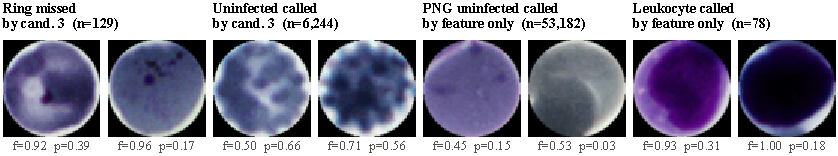
\includegraphics[width=\textwidth]{figures/fig_failures.pdf}
\caption{BBBC041 errors on ellipse crops, two drawn at random (fixed seed) from each category; $n$ is the category size. $f$: dark-spot score (threshold 0.3047); $p$: candidate 3's ensemble probability (threshold 0.5).}
\label{fig:failures}
\end{figure*}

\subsection{Prediction record}
\label{sec:record}
Table~\ref{tab:record} lists our main predictions. Only four of these 15 predictions were fully supported. The session-leakage prediction failed its registered rule on the point estimate, but its CI contains both zero and the predicted value, so the result is unresolved rather than refuted. The misses are informative: we overestimated leakage, overestimated colour augmentation on NIH, underestimated colour transfer externally, underestimated seed variance, and overestimated a simple rule's ability to transfer.

\begin{table}[t]
\caption{Main predictions and outcomes}
\label{tab:record}
\centering
\scriptsize
\setlength{\tabcolsep}{2.5pt}
\begin{tabular}{@{}L{0.26\columnwidth}L{0.38\columnwidth}L{0.28\columnwidth}@{}}
\toprule
Experiment & Prediction & Outcome \\
\midrule
Leakage (M3) & BACC drops 1--2.5\pp{} on unseen patients & \textbf{Missed}: drop of 0.23--0.26 \\
ColorJitter (M3) & BACC $+0.3$ to $+1.0$ on unseen patients & \textbf{Falsified}: $-0.04$ \\
Probes & BACC 75--93\% & \textbf{Missed}: 96.0--96.5 \\
Explanations (5 ckpts) & Darkest pixel beats Grad-CAM & \textbf{Supported}: 15/15 \\
Norm layer replication & LayerNorm gains more from leakage & \textbf{Not replicated} \\
Colour transfer, MP-IDB & Little change & \textbf{Falsified}: $+7.05$ \\
Test-time Reinhard & BACC $+2$ to $+6$ & \textbf{Falsified}: $-18.75$ \\
Session leakage & Gap about $+0.35$ & \textbf{Not supported}: $+0.24$ [$-0.06$, $0.59$]; CI holds 0 and $+0.35$ \\
Seed variance & SD 3--6 on MP-IDB & \textbf{Missed high}: 6.63 \\
NIH seed SD & Under 0.5, $\le$1/5 of MP-IDB & \textbf{Supported}: 0.18 \\
No attention & BACC $-0.5$ to $-2.5$, CI below 0 & \textbf{Supported}: $-0.74$ \\
Max-pool head & $|\Delta|<0.29$, CI includes 0 & \textbf{Missed}: $-0.19$, CI excludes 0 \\
BBBC041 outcome & Feature holds (45\%) & \textbf{Wrong}: trained wins \\
BBBC041 rule BACC & 78--90 & \textbf{Missed}: 61.3 \\
BBBC041 leukocytes & Rule flags $\ge$60\% & \textbf{Supported}: 99\% \\
\bottomrule
\end{tabular}\\[2pt]
\raggedright\scriptsize Milestone 3 rows were dated externally (2026-10-05); other dates are self-reported. Full record and corrections are in the project registry.
\end{table}

% =====================================================================
\section{Discussion}
\textbf{NIH accuracy mostly measures a strong, simple cue.} On curated NIH crops, the parasite is usually the darkest object in a pale cell. One darkness measurement reached AUC 0.981; a generic ResNet-18, frozen probes and a 43k-parameter DANet without attention all came within a point of it; leakage at patient and session level was below our detection limit; and Grad-CAM pointed at the parasite less reliably than the darkest pixel. None of this shows that DANet is poor. It shows that a 97\% score on NIH says little about \emph{what} a model has learned.

\textbf{Transfer depends on the operating point, and NIH cannot reveal it.} On BBBC041 the gap between trained ensembles and the rule grew from about one point to 25--31 points. Most of that came from thresholds, not ranking: the rule kept AUC above 0.90 and nearly matched the ensembles on the JPG group, but its NIH threshold failed on the PNG group. Trained models showed the same split on MP-IDB, where their ranking was stable across crop masks while their balanced accuracy moved by 12 points. External validation should therefore report threshold-free and fixed-threshold results together.

\textbf{Colour transfer is a likely, but unisolated, contributor outside NIH.} Colour augmentation did nothing on unseen NIH patients, while training-time colour transfer raised MP-IDB accuracy by seven points in a controlled comparison. On BBBC041 the colour-transfer ensemble was the only candidate with balanced errors and the only one to reject most leukocytes, but it differs from the plain DANet ensemble in three ways at once: colour transfer, 20 members rather than 5, and a mix of architectures (three DANet variants and ResNet-18). Its margin over candidate 2 ($+0.011$ AUC [0.007, 0.017]) therefore cannot be credited to colour transfer alone. Our Milestone~3 intuition that stain matters may be right for new sources, but this study does not establish it.

\textbf{Development data misled us.} MP-IDB was reused for many decisions, including the rule's design, and rehearsal there favoured the rule on ellipse crops. BBBC041 reversed that. Seed variance (Fig.~\ref{fig:seeds}) adds a second warning: on one fixed training set, a new seed alone moved external accuracy across 18 points. External claims should rest on data untouched by development, with ensembles or many checkpoints, and candidates frozen before scoring.

\section{Limitations}
This study makes no clinical claim. PPV at BBBC041's natural prevalence was 13--26\% at best, far from a usable screening test, and curated cell crops are not a field workflow. Species, stain and acquisition change together between datasets, so we cannot assign a transfer failure to one cause. BBBC041 is a single external dataset with one dominant acquisition group. BBBC041 provides boxes, not masks, and our crop audit was done by an AI assistant, not a microscopist. Session leakage rests on one repeat, and image date is only a proxy for session. Prediction dates after Milestone~3 are self-reported. We excluded red-cell boxes that overlap a parasite box (4{,}344), which removes some hard negatives and may make specificity look better than it would on every cell. Candidates 2 and 3 differ in more than colour transfer (Section~\ref{sec:bbbc}). The architecture ablation used one seed per arm. Finally, our explanation analysis tested one method, Grad-CAM.

\section{Conclusion}
We reproduced DANet within its own reported range, falsified our own hypothesis that colour augmentation would help on unseen NIH patients, and found that NIH's 97\% rests largely on a cue that one measurement captures. Retraining with a new seed alone moved external accuracy by several points while NIH stayed flat. In a frozen one-shot test on BBBC041, a colour-transfer ensemble beat the one-measurement rule by 25--31 points of balanced accuracy, because the rule's NIH threshold did not transfer. Benchmarks like NIH should be reported with patient-grouped splits, simple baselines, several checkpoints and, above all, a frozen test on data that played no part in development.

\section*{Acknowledgment}
We thank our course instructors for the reproduction framework. \textbf{Use of AI.} An AI assistant (Claude, Anthropic) helped design experiments, write code, draft predictions after Milestone~3, run analyses, verify references and draft this text. The Milestone~3 hypothesis was submitted by the authors on 2026-10-05. The authors reviewed every result. Code, splits, predictions and the full registry are kept in the project repository.

\bibliographystyle{IEEEtran}
\bibliography{refs}

\end{document}
